Organize this section according to the rules defined in the project description. 
\subsection{External Interface Requirements}
\subsubsection{User Interfaces}
\subsubsection{Hardware Interfaces}
\subsubsection{Software Interfaces}
\subsubsection{Communication Interfaces}

\subsection{Functional Requirements}
\begin{enumerate}
\item[•]{\Large Data4Help}
	\begin{enumerate}
	\item [G.1] \textbf{Collect users' position and health status.}
		\begin{enumerate}
		\item [D.1] Users' information are collected from partner applications or from the other two TrackMe applications installed on users' devices.
		\item [D.2] All the partner applications require to submit user credentials.
		\item [D.3] The identification (fiscal code, social security number) and the secondary data (attributes) given by the individual during the registration are correct.
		\item [R.1] Retrieve user credentials inserted into partner application as group attributes.
		\item [R.2] Allow users already registered in Data4Help world to sign in with his account without provide user credentials again.
		\item [R.3] Allow individuals to agree with privacy policy (first part). Registered users, now, can be tracked in group mode request through installed application.  
		\item [R.4] Allow individuals to specify, during registration, if they are also interested to be tracked in single mode request (second part) through installed application.  .
		\item [D.4] Devices used to monitor individuals always work and report 			the correct values.	
    	\item [D.5] Partner application always report correct values to Data4Help.
    	\item [R.5] The system has to correctly receive data from partner applications installed on users' device.
    	\end{enumerate}	
    	
    \item [G.2] \textbf{Provide to Third Parties, the users' position and heath status.}
    	\begin{enumerate} 
    	\item [R.6] Allow third parties registration to Data4Help service, where they have to specify all their credentials.
    	\end{enumerate}	
		
		\begin{enumerate} 
		\item [G.2.1] \textbf{Provide data on-demand to non-subscribed third parties.}
		\begin{enumerate} 
		\item [R.7] For each user registered ,the system has to automatically retrieve and store data from partner applications with a resolution of 10 minutes; independently from the requests reached.	
		\item [R.8] The system has to collect inside his database all the useful information that match the request.
		\item [R.9] The system has to send to applicant all the data already collected.
    	\end{enumerate}	
    	
    	\item [G.2.2] \textbf{Provide data in real-time to subscribed third parties.}
		\begin{enumerate}
		\item [D.8] Live acquisition lasts 24 hours to reduce waste of resources.
    	\item [R.10] Allow third parties subscription to interested group in order to receive live data.
    	\item [R.11] When a real time request is performed the system has to collect and store specific users' data with a resolution of 1 minute.
    	\item [R.12] Provide to subscribed third parties data as soon as they are available by the system.
    	\end{enumerate}
    	\end{enumerate}
    
	\item [G.3] \textbf{Allow third parties two different ways to get users' data.}
		\begin{enumerate}     
    	\item [G.3.1] \textbf{Allow third parties to get data of a single person.}
		\begin{enumerate}
		\item [D.6] In order to perform an individual request, third parties has to know the user's fiscal code or security number.
		\item [D.7] Security number and fiscal code are not information given to third parties by Data4Help.
    	\item [R.13] Allow third parties to insert fiscal code of user that want to track.
    	\item [R.14] Deny third parties to receive information about users in  single mode, that have not accepted second part of privacy policy.
    	\item [R.15] Collect all the useful information retrieved by Data4Help that are produced by the interested users 
    	\item [R.16] Send all the collected information to request applicant.
    	\end{enumerate}
    
    	\item [G.3.2] \textbf{Allow third parties to get data of a group of people.}
		\begin{enumerate}
    	\item [R.17] Allow third parties to insert attributes in which they are interested to restrict their field of search.
    	\item [R.18] Deny third parties to receive information if the provided information can hurt users' privacy, for this purpose group request under 1000 users involved are rejected.
    	\item [R.15] Collect all the useful information retrieved by Data4Help that are produced by the interested users 
    	\item [R.16] Send all the collected information to request applicant.
    	\end{enumerate}
    	\end{enumerate}
    	
    \item [G.4] \textbf{Provide data in an anonymous way, to protect users' privacy.}
		\begin{enumerate}
    	\item [R.14] Deny third parties to receive information about users in  single mode, that have not accepted second part of privacy policy.
    	\item [R.18] Deny third parties to receive information if the provided information can hurt users' privacy, for this purpose group request under 1000 users involved are rejected.
    	\end{enumerate}	
			
	\end{enumerate}
	
	
\item[•]{\Large AutomatedSOS}
	
	\begin{enumerate}
	\item [G.5] \textbf{Retrieve user's position and health status.}
		\begin{enumerate}
		\item [R.19] Allow users to be tracked from AutomatedSOS filling up the registration and agreeing to both parts of privacy policy.
		\item [D.4] Devices used to monitor individuals always report correct values.
		\item [D.9] The user always dresses a smartwatch on which AutomatedSOS is installed.    
		\item [R.20] The application has to interact with Smartwatch/Smartphone APIs in order to retrieve location and health status.
		\item [R.21] The application is able to send to Data4Help service all the informations already retrieved in live acquisition.
		\end{enumerate}
		
	\item [G.6] \textbf{Allow health-interested third parties the access to data detected by AutomatedSOS.}
		\begin{enumerate}
		\item [R.22] Allow non-profit organizations to register into AutoatedSOS portal and becoming health third parties.
		\item [R.23] Allow health third parties to receive informations about all the users registered to AutomatedSOS through Live Acquisition performed by Data4Help.
		\end{enumerate}
	
	\item [G.7] \textbf{Monitor user's health parameters.}
		\begin{enumerate}
		\item [R.20] The application has to interact with Smartwatch/Smartphone APIs in order to retrieve location and health status.
		\end{enumerate}
		
	\item [G.8] \textbf{Send an ambulance to users' location whenever certain parameters are below the threshold.}
		\begin{enumerate}
		\item [R.24] The application has to control health status with data retrieved in local to realize immediately if certain parameters are critical.
		\item [R.25] The application has to call an ambulance, if parameters are critical.
		\item [D.10] The ambulance system is always up and ready to receive messages from AutomatedSOS.
		\item [R.26] Supply to hospital user's location and all the useful information to provide efficient first aid.
		\item [D.11] The ambulance successfully reach the location of the individual.
		\end{enumerate}
		
  	\end{enumerate}
  	
  	
\item[•]{\Large Track4Run}
	
	\begin{enumerate}
	\item [G.5] \textbf{Retrieve user's position and health status.}
		\begin{enumerate}
		\item [R.27] Allow users to be tracked from Track4Run filling up the registration and agreeing to both parts of privacy policy.
		\item [D.4] Devices used to monitor individuals always report correct values.
		\item [R.20] The application has to interact with Smartwatch/Smartphone APIs in order to retrieve location and health status.
		\item [R.21] The application is able to send to Data4Help service all the informations already retrieved in live acquisition.
		\end{enumerate}
		
	\item [G.9] \textbf{Allow promoters to manage a run.}
		\begin{enumerate}
		\item [R.22] Allow users to create a run providing all the general information about the competition.
		\item [R.23] Allow users to specify if the race is public or private.
		\item [D.4] Devices used to monitor individuals always report correct values.
		\item [D.13] During a run athletes always dress a smartwatch on which Track4Run is installed.
			
		\item [G.9.1] \textbf{Allow promoters to define a path for the run.}
			\begin{enumerate}
			\item [R.24] Allow promoters to define a path for the race by selecting the routes inside a map.
			\item [D.14] The path defined by the organizer actually exist.
			\end{enumerate}
			
		\item [G.9.2] \textbf{Allow promoters to invite athletes to the run.}
			\begin{enumerate}
			\item [R.25] Allow promoters to invite athlete to be runner of their private race.
			\item [R.26] Allow promoters to specify maximum number of athletes that can take part to their public race.
			\end{enumerate}
	\end{enumerate}
	
	\item [G.10] \textbf{Allow athletes to enroll on a specific run.}
		\begin{enumerate}
		\item [R.27] Allow users to see all the public races and private races in which he is invited.
		\item [R.28] Allow user to select a race and add him to the athletes involved.
		\item [D.16] If an athlete enroll to a run then he also participates to the run.
		\end{enumerate}
	
	\item [G.11] \textbf{Allow spectators to watch in real time the position of every athletes in a specific run.}
		\begin{enumerate}
		\item [D.17] All athletes have their tracking devices with them and the application enabled for the entire duration of the run.	
		\item [R.29] Allow user to select a race to be viewed.
		\item [R.30] The application must be able to request to Data4Help the positions of all the other athletes involved.
		\item [R.31] The application must be able to receive and display the positions of all the other athletes involved.
		\item [D.18] Athletes never go out of the defined path.
		\end{enumerate}
	\end{enumerate}

\end{enumerate}

\subsubsection{Use Case Diagram}

\begin{enumerate}

\FloatBarrier
\item[•]{\Large Data4Help Use Cases}

\begin{table}[h]
\begin{tabular}{|l|l|}
\hline
Name             & Sign up \\ \hline
Actors           & Third Party  \\ \hline
Entry Conditions & The third party has the registration website page opened.    \\ \hline
Event Flow       & \parbox{.45\textwidth}{\begin{enumerate}
            \item The third party clicks on the "Sing Up" button.
            \item The third party fills all the attribute fields and clicks on "Register Now" button.
            \item The system creates the third party's account saving its attributes.
        \end{enumerate}}\\ \hline
Exit Condition   & The third party's account has been created and the third party is now registered.\\ \hline
Exceptions       & \parbox{.45\textwidth}  
{\begin{itemize}
\item If the system notices that attributes used in the registration are already linked to an existing account then a warning is generated saying that there is already a third party registered with the given credentials.
\end{itemize}}\\ \hline
\end{tabular}
\end{table}
\FloatBarrier

\FloatBarrier
\begin{table}[h]
\begin{tabular}{|l|l|}
\hline
Name             & Sign in \\ \hline
Actors           & Third Party  \\ \hline
Entry Conditions & The third party has the registration website page opened.    \\ \hline
Event Flow       & \parbox{.45\textwidth}{\begin{enumerate}
            \item The third party clicks on the "Sing In" button.
            \item The third party fills all credentials fields and clicks on "Log in" button.
            \item The system accept the login request.
        \end{enumerate}}\\ \hline
Exit Condition   & The third party's account has been loaded by the website and the user is now logged in.\\ \hline
Exceptions       & \parbox{.45\textwidth}  
{\begin{itemize}
\item If user inserts invalid log in credentials a warning is generated, saying the credentials are invalid.
\end{itemize}}\\ \hline
\end{tabular}
\end{table}
\FloatBarrier

\FloatBarrier
\begin{table}[h]
\begin{tabular}{|l|l|}
\hline
Name             & Request Individual Monitoring \\ \hline
Actors           & Third Party  \\ \hline
Entry Conditions & The third party is logged in.    \\ \hline
Event Flow       & \parbox{.45\textwidth}{\begin{enumerate}
            \item The third party clicks on the "Individual Request" button.
            \item The third party inserts the fiscal code or the social security number of the individual to track .
            \item The system shows the outcome of the request. 
        \end{enumerate}}\\ \hline
Exit Condition   & The request's outcome is shown.\\ \hline
Exceptions       & \parbox{.45\textwidth}  
{\begin{itemize}
\item If the inserted fiscal code or social security number are not linked to any Account then a warning message is displayed, saying that the individual is not registered.
\item If the individual with the fiscal code or social security number inserted didn't accept the individual treatment of data policy then a warning message is displayed. This message says that the request is rejected.
\item If the individual with the fiscal code or social security number inserted did accept the individual treatment of data policy then a message is displayed saying that the individual have accepted the request and all his data collected until the moment of the request are shown to the third party.
\end{itemize}}\\ \hline
\end{tabular}
\end{table}
\FloatBarrier

\FloatBarrier
\begin{table}[h]
\begin{tabular}{|l|l|}
\hline
Name             & Request Group Monitoring \\ \hline
Actors           & Third Party  \\ \hline
Entry Conditions & The third party is logged in.    \\ \hline
Event Flow       & \parbox{.45\textwidth}{\begin{enumerate}
            \item The third party clicks on the "Group Request" button.
            \item The third party inserts the all the attributes that will define the group of interest.
            \item The system shows the outcome of the request. 
        \end{enumerate}}\\ \hline
Exit Condition   & The request's outcome is shown.\\ \hline
Exceptions       & \parbox{.45\textwidth}  
{\begin{itemize}
\item If the group is made by less than 1000 individuals the request is rejected and a the outcome is shown in a form of a warning saying that the request got rejected.
\end{itemize}}\\ \hline
\end{tabular}
\end{table}
\FloatBarrier

\FloatBarrier
\begin{table}[h]
\begin{tabular}{|l|l|}
\hline
Name             & Subscribe To A Group\\ \hline
Actors           & Third Party  \\ \hline
Entry Conditions & The third has just sent an accepted monitoring request to a group. \\ \hline
Event Flow       & \parbox{.45\textwidth}{\begin{enumerate}
            \item The third party clicks on the "Subscribe to this Group" button.
            \item The system from now on will always send to the third party new data about this group.
            \item 
        \end{enumerate}}\\ \hline
Exit Condition   & The third party is subscribed to the selected group.\\ \hline
Exceptions       & None \\ \hline
\end{tabular}
\end{table}
\FloatBarrier


\item[•]{\Large AutomatedSOS Use Cases}
\FloatBarrier
\begin{table}[h]
\begin{tabular}{|l|l|}
\hline
Name             & Sign up \\ \hline
Actors           & User  \\ \hline
Entry Conditions & The User has AutomatedSOS application installed on his/her smartwatch.    \\ \hline
Event Flow       & \parbox{.45\textwidth}{\begin{enumerate}
            \item The user clicks on the "Sing Up" button.
            \item The user accepts the treatment of data policy.
            \item The user fills all the attribute fields and clicks on "Register Now" button.
            \item The system creates the user's account saving his/her attributes.
        \end{enumerate}}\\ \hline
Exit Condition   & The user's account has been created and the user is now registered.\\ \hline
Exceptions       & \parbox{.45\textwidth}  
{\begin{itemize}
\item If the user does not accept the treatment of data policy a warning is generated saying that in order to register the policy must be accepted.
\item If the system notices that the social security number or fiscal code used in a registration are already linked to an existing account then a warning is generated saying that there is already an account registered with the given credentials.
\end{itemize}}\\ \hline
\end{tabular}
\end{table}
\FloatBarrier

\FloatBarrier
\begin{table}[h]
\begin{tabular}{|l|l|}
\hline
Name             & Sign in \\ \hline
Actors           & User  \\ \hline
Entry Conditions & The User has AutomatedSOS application installed on his/her smartwatch.    \\ \hline
Event Flow       & \parbox{.45\textwidth}{\begin{enumerate}
            \item The user clicks on the "Sing In" button.
            \item The user inserts his/her social security number or fiscal code and his/her password, then clicks the "Enter" button.
            \item The system accept the login in request.
        \end{enumerate}}\\ \hline
Exit Condition   & The user's account has been loaded by the app and the user is now logged in.\\ \hline
Exceptions       & \parbox{.45\textwidth}  
{\begin{itemize}
\item If user inserts invalid log in credentials a warning is generated, saying the credentials are invalid.
\end{itemize}}\\ \hline
\end{tabular}
\end{table}
\FloatBarrier

\FloatBarrier
\begin{table}[h]
\begin{tabular}{|l|l|}
\hline
Name             & Monitor data \\ \hline
Actors           & User  \\ \hline
Entry Conditions & The User is logged in. \\ \hline
Event Flow       & \parbox{.45\textwidth}{\begin{enumerate}
            \item The user clicks on the "Monitor Data" button.
            \item The system gets all the information that have been retrieved by the application to the user.
\end{enumerate}}\\ \hline
Exit Condition   & All the information retrieved by the application are shown on the app.\\ \hline
Exceptions       & \parbox{.45\textwidth}  
{\begin{itemize}
\item If the system do not find information about the user then a warning message is shown to the user saying that until now no user data has been recorded by the application.
\end{itemize}}  \\ \hline
\end{tabular}
\end{table}
\FloatBarrier

\FloatBarrier
\begin{table}[h]
\begin{tabular}{|l|l|}
\hline
Name             & Monitor current health status \\ \hline
Actors           & User  \\ \hline
Entry Conditions & The User is logged in. \\ \hline
Event Flow       & \parbox{.45\textwidth}{\begin{enumerate}
            \item The user clicks the "Monitor health status" button.
            \item The system shows all the health values that are being retrieved in real time.
        \end{enumerate}}\\ \hline
Exit Condition   & All the health parameters retrieved by the application are shown on the app in real time.\\ \hline
Exceptions       & \parbox{.45\textwidth}  
{\begin{itemize}
\item If no health parameters are retrieved a warning message is displayed saying to the user he must wear the smartwatch in order to see parameters in real time. \end{itemize}}\\ \hline
\end{tabular}
\end{table}
\FloatBarrier

\FloatBarrier
\begin{table}[h]
\begin{tabular}{|l|l p{3cm}|}
\hline
Name             & Send Ambulance Request \\ \hline
Actors           & AutomatedSOS, Croce Rossa  \\ \hline
Entry Conditions & A critical health parameter value is below the threshold. \\ \hline
Event Flow       & \parbox{\textwidth}{\begin{enumerate}
            \item AutomatedSOS send to "Croce Rossa" a form that contains all important information about the user, like his current location, his gender, his age, her health profile, and the list of parameters below the threshold.
            \item Croce Rossa send an acknowledge message to AutomatedSOS and send immediately an ambulance to the user location.
            \item AutomatedSOS displays on the app a warning message saying that an ambulance is currently heading to the user's location. 
        \end{enumerate}}\\ \hline
Exit Condition   & \parbox{\textwidth}{A warning message is shown saying that an ambulance is currently heading to the user's location. OR . The ambulance reaches the user's location. OR . The ambulance is traveling to the user's location.} \\ \hline
Exceptions       & \parbox{\textwidth}  
{\begin{itemize}
\item If no acknowledge message is received by AutomatedSOS after the form has been sent, as soon as a certain time out expires AutomatedSOS resend the form with updated information. \end{itemize}}\\ \hline
Special Requirements   & The form need to be sent to "Croce Rossa" with a reaction time of less than 5 seconds from the time the parameters are below the threshold. \\ \hline
\end{tabular}
\end{table}
\FloatBarrier

\FloatBarrier
\item[•]{\Large Track4Run Use Cases}
\begin{table}[h]
\begin{tabular}{|l|l|}
\hline
Name             & Sign up \\ \hline
Actors           & User  \\ \hline
Entry Conditions & The User has Track4Run application installed on his/her smartwatch.    \\ \hline
Event Flow       & \parbox{.45\textwidth}{\begin{enumerate}
            \item The user clicks on the "Sing Up" button.
            \item The user accepts the treatment of data policy.
            \item The user fills all the attribute fields and clicks on "Register Now" button.
            \item The system creates the user's account saving his/her attributes.
        \end{enumerate}}\\ \hline
Exit Condition   & The user's account has been created and the user is now registered.\\ \hline
Exceptions       & \parbox{.45\textwidth}  
{\begin{itemize}
\item If the user does not accept the treatment of data policy a warning is generated saying that in order to register the policy must be accepted.
\item If the system notices that the social security number or fiscal code used in a registration are already linked to an existing account then a warning is generated saying that there is already an account registered with the given credentials.
\end{itemize}}\\ \hline
\end{tabular}
\end{table}
\FloatBarrier

\FloatBarrier
\begin{table}[h]
\begin{tabular}{|l|l|}
\hline
Name             & Sign in \\ \hline
Actors           & User  \\ \hline
Entry Conditions & The User has Track4Run application installed on his/her smartwatch or smartphone.    \\ \hline
Event Flow       & \parbox{.45\textwidth}{\begin{enumerate}
            \item The user clicks on the "Sing In" button.
            \item The user inserts his/her social security number or fiscal code and his/her password, then clicks the "Enter" button.
            \item The system accept the login in request.
        \end{enumerate}}\\ \hline
Exit Condition   & The user's account has been loaded by the app and the user is now logged in.\\ \hline
Exceptions       & \parbox{.45\textwidth}  
{\begin{itemize}
\item If user inserts invalid log in credentials a warning is generated, saying the credentials are invalid.
\end{itemize}}\\ \hline
\end{tabular}
\end{table}
\FloatBarrier

\FloatBarrier
\begin{table}[h]
\begin{tabular}{|l|l|}
\hline
Name             & Promote a run \\ \hline
Actors           & User  \\ \hline
Entry Conditions & The User is logged in.    \\ \hline
Event Flow       & \parbox{.45\textwidth}{\begin{enumerate}
            \item The user clicks on the "Promote a Run" button.
            \item The system show a new tab where the user can define the path, name, date and athletes (other users).
            \item The system create the event and automatically send notifications to all athletes specified by the promoter asking them if they want to participate to the run.
        \end{enumerate}}\\ \hline
Exit Condition   & The run event has been created and is visible in the list of promoted events.\\ \hline
Exceptions       & \parbox{.45\textwidth}  
{\begin{itemize}
\item During the creation of the run the user can cancel the operation and go back to the main menu at any point clicking the "Cancel" button.
\item If the user do not insert critical information like the path, the name and the date a warning message is shown saying that critical parameters are missing in order to create the run. The user can close the warning message and fill the remaining parameters or cancel the operation, going back to the main menu.
\item The system needs to do something if the defined path cannot be a real path for the run??
\end{itemize}}\\ \hline
\end{tabular}
\end{table}
\FloatBarrier

\FloatBarrier
\begin{table}[h]
\begin{tabular}{|l|l|}
\hline
Name             & Enroll to a run \\ \hline
Actors           & User  \\ \hline
Entry Conditions & The User is logged in.    \\ \hline
Event Flow       & \parbox{.45\textwidth}{\begin{enumerate}
            \item The user clicks on the "Enroll to a Run" button.
            \item The system shows a new tab where the list of all runs created is visible.
            \item The user can filter the runs with attributes like the name, the date and the location.
            \item The user clicks the "Enroll" button associated to the specific run.
            \item The system add the user to the list of athletes enrolled to the run.
        \end{enumerate}}\\ \hline
Exit Condition   & The user is inside the list of athletes.\\ \hline
Exceptions       & \parbox{.45\textwidth}  
{\begin{itemize}
\item If the number of athletes has already capped the max amount in a specific run then the user cannot click on the "Enroll" button associated to that run.
\item How to see if the athlete actually has a smartwatch??
\end{itemize}}\\ \hline
\end{tabular}
\end{table}
\FloatBarrier

\FloatBarrier
\begin{table}[h]
\begin{tabular}{|l|l|}
\hline
Name             & Spectate a run \\ \hline
Actors           & User  \\ \hline
Entry Conditions & The User is logged in.    \\ \hline
Event Flow       & \parbox{.45\textwidth}{\begin{enumerate}
            \item The user clicks on the "Spectate a Run" button.
            \item The system shows a new tab where the list of all live runs is visible.
            \item The user can filter the runs with attributes like the name, and the location.
            \item The user clicks the "Spectate" button associated to the specific run.
            \item The system opens a tab which contains the path of the run and also the position of all athletes in real time.
        \end{enumerate}}\\ \hline
Exit Condition   & The spectator tab on the application is open.\\ \hline
Exceptions       & \parbox{.45\textwidth}  
{\begin{itemize}
\item What if there is a maximum amount of spectator to a run?
\end{itemize}}\\ \hline
\end{tabular}
\end{table}
\FloatBarrier

\end{enumerate}

\subsection{Sequence Diagram}
\begin{enumerate}
\item[•]{\Large Data4Help}



\begin{minipage}{\textwidth}
\FloatBarrier
Individual request with on-demand acquisition performance.
\begin{center}
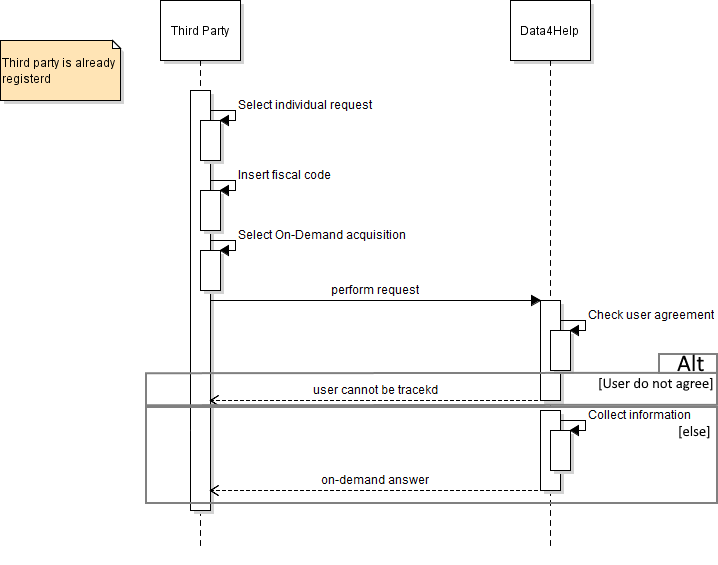
\includegraphics[scale=0.8]{Images/Seq_Data4Help_onDem.png}
\end{center}
\FloatBarrier

\FloatBarrier
Automatic data update inside Data4Help.
\begin{center}
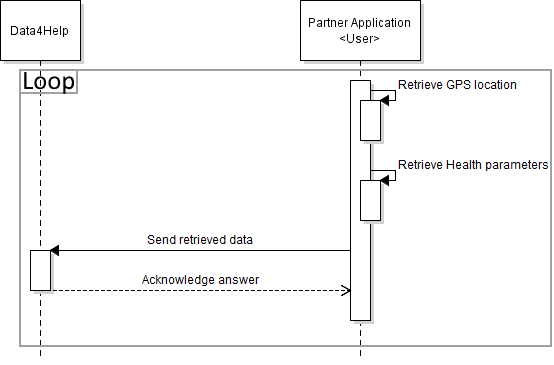
\includegraphics[scale=0.8]{Images/Seq_Data4Help_autoUp.png}
\end{center}
\FloatBarrier

\end{minipage}

\begin{minipage}{\textwidth}
\FloatBarrier
Group request with live acqusition performance
\begin{center}
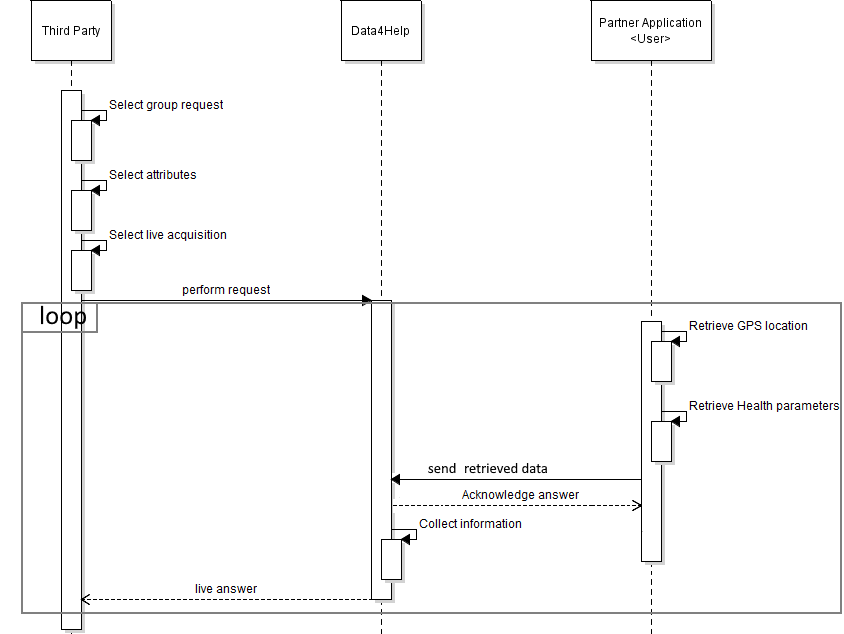
\includegraphics[scale=0.75]{Images/Seq_Data4Help_live.png}
\end{center}
\FloatBarrier
\end{minipage}


%Two images side by side
%\begin{figure}[htbp]
%  \begin{minipage}[b]{0.5\linewidth}
%    \centering
%    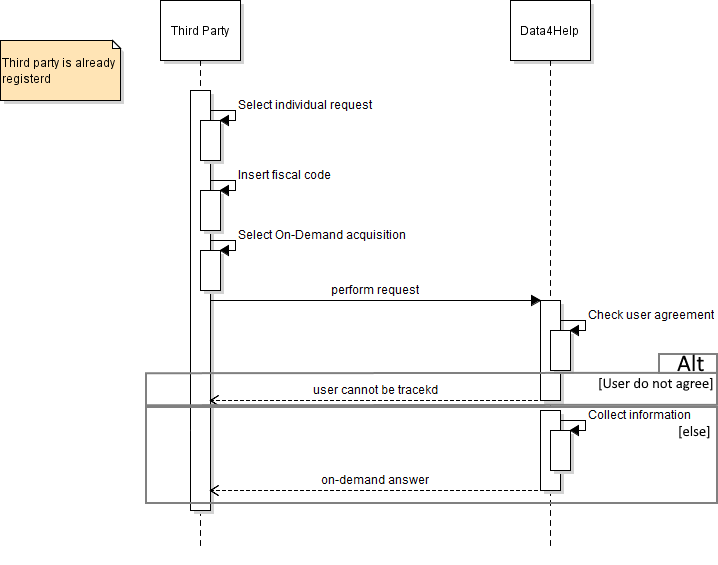
\includegraphics[width=\linewidth]{Images/Seq_Data4Help_onDem.png}
%    \caption{The caption for figure 1}
%    \label{fig:chapter001_dist_001}
%  \end{minipage}
%  \hspace{0.5cm}
%  \begin{minipage}[b]{0.5\linewidth}
%    \centering
%    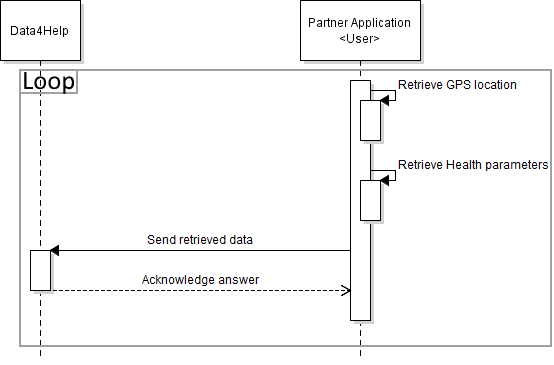
\includegraphics[width=\linewidth]{Images/Seq_Data4Help_autoUp.png}
%    \caption{The caption for figure 2.}
%    \label{fig:chapter001_reward_001}
%  \end{minipage}
%\end{figure}





\end{enumerate}



\subsection{Performance Requirements}

\subsection{Design Constraints}
\subsubsection{Standards compliance}
\subsubsection{Hardware limitations}
\subsubsection{Any other constraint}

\subsection{Software System Attributes}
\subsubsection{Reliability}
\subsubsection{Availability}
\subsubsection{Security}
\subsubsection{Maintainability}
\subsubsection{Portability}
